%1. Grundlagen
\chapter{Grundlagen}
Diese Studienarbeit befasst sich mit dem komplexen Thema der Elliptischen Kurven in der Kryptographie. Die Kryptographie ist ein stark mathematisches Thema, bei welchem es zu Anfang der Legung einer Grundlage für das Verständnis der Inhalte dieser Studienarbeit. In diesem Kapitel werden sowohl die mathematischen als auch die kryptographischen Grundlagen zum Verständnis der in dieser Arbeit behandelten Elliptischen Kurven der Charakteristik p>3 gelegt. 

\begin{figure}[!h]
\centering
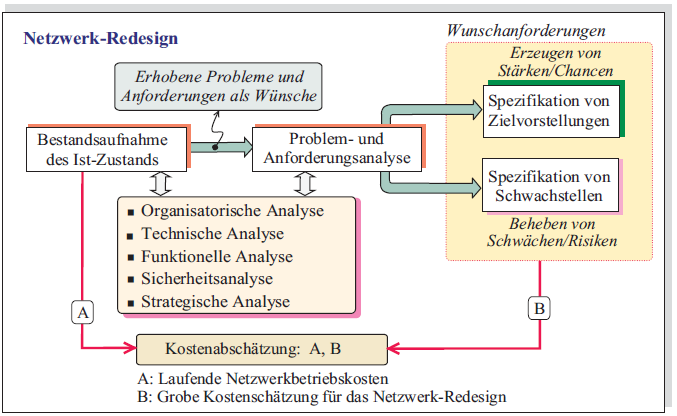
\includegraphics[width=\textwidth]{grafiken/aufgaben_redesign.png}
\caption[Hauptaufgaben der Ist-Analyse beim Redesign einer Netzwerkinfrastruktur]{Hauptaufgaben der Ist-Analyse beim Redesign einer Netzwerkinfrastruktur \\ Quelle: \cite{Berghammer.2021}}
\label{fig:aufgaben_redesign}
\end{figure}

\section{Primzahlen}
XXX

\subsection{Definition}
x

\subsection{Eigenschaften}
x

\subsection{Bestimmung von Primzahlen}
x

\subsection{Rolle der Primzahlen in der Kryptologie}
x

\section{Algebraische Strukturen}
Definiert durch die Zahlentheorie und als zentraler Untersuchungsgegenstand des mathematischen Teilgebietes der universellen Algebra, liefern algebraische Strukturen die Basis zur Realisierung komplexer symmetrischer und asymmetrischer Kryptosysteme, weshalb wir im folgenden Kapitel die Eigenschaften relevanter algebraischer Strukturen näher betrachten wollen. Darüber hinaus möchten wir Ihnen auch einige Werkzeuge zum Rechnen in der jeweiligen algebraischen Struktur an die Hand geben, welche zur späteren Realisierung von Kryptosystemen benötigt werden.\\

Unter einer sehr allgemeinen Betrachtung ist eine mathematische Struktur eine Liste nichtleerer Mengen, genannt Trägermengen, mit Elementen aus den Trägermengen, genannt Konstanten, und mengentheoretischer Konstruktionen über den Trägermengen. Diese sind konkret Funktionen über den Trägermengen.
Im Weiteren beschränken wir uns auf den Fall einer einzigen Trägermenge, wodurch die Strukturen als homogen bezeichnet werden können.
\paragraph{Definition: Homogene algebraische Struktur}
Eine homogene algebraische Struktur ist ein Tupel $(M,c_1,\dots,c_m,f_1,\dots,f_n)$ mit $m,n \in \mathbb{N}$ und $n \geq 1$. Dabei ist $M$ eine nichtleere Menge, genannt \textbf{Trägermenge}, alle $c_i$ sind Elemente aus $M$, genannt die \textbf{Konstanten}, und alle $f_i$ sind $s_i$-stellige Funktionen $f_i:M \rightarrow M$ im Fall $s = 1$ und $f_i:M^{s_i} \rightarrow M$ im Fall $s_i>1$, genannt die (inneren) \textbf{Operationen}. Die lineare Liste$(0,\dots,0,s_1,\dots,s_n)$ mit $m$ Nullen heißt \textbf{Typ} oder die \textbf{Signatur}.\newline

Laut dieser Definition muss eine homogen algebraische Struktur nicht unbedingt Konstanten enthalten, jedoch mindestens eine Operation. Das Paar $(\mathbb{N},+)$ bildet beispielsweise eine homogene algebraische Struktur des Typs (2). Das 5-Tupel $(\mathbb{N},0,1,+,\cdot)$ bildet ebenfalls eine homogen algebraische Struktur des Typs (0,0,2,2).

Algebraische Strukturen unterscheiden sich grundsätzlich durch ihren Typ. Wirklich charakterisiert werden sie aber erst durch die jeweils geltenden Axiome, d.h. bestimmte Eigenschaften, welche für die Konstanten und Operationen gefordert werden. Durch die Hinzunahme immer weiterer Axiome, entsteht eine Hierarchie immer feinerer Strukturen, an deren Anfang der Monoid steht.

\subsection{Monoid}
\paragraph{Definition: Monoid}
Eine algebraische Struktur $(M,e,\cdot)$ des Typs (0,2) heißt ein Monoid, falls für alle $x,y,z\in M$ die folgenden Monoid Aciome gelten: $$x \cdot (y \cdot z) = (x \cdot y) \cdot z$$ $$ e \cdot x = x = x \cdot e$$ Gilt zusätzlich noch für alle $x,y \in M$ die Gleichung $x \cdot y = y \cdot x$, so heiß $(M,e,\cdot)$ ein \textbf{kommutatives Monoid}.

Die erste und die letzte Gleichung bilden das Assoziativ- und Kommutativgesetz ab. Durch die mittlere Gleichung wird ein neutrales Element $e$ bezüglich der Operation gefordert, wobei sowohl die \textbf{Linksneutralität} als auch die \textbf{Rechtsneutralität} spezifiziert wird.

Beispiele für Monoide sind $(\mathbb{N},0,+)$, $(\mathbb{N},1,\cdot)$ und $(\mathbb{Z},0,+)$.

\subsubsection{Gruppe}
\subsubsection{Ring}
\subsubsection{Körper}

\section{Allgemeines zur Verschlüsselung}
XXX

\subsection{Symmetrische und Asymmetrische Verschlüsselung}
x

\subsection{Diffie-Hellmann}
x

\section{Ziel der Arbeit}
XXX

\section{Geplante Vorgehensweise}
XXX